\topic{Integral Domains}

Keep in mind \((\Z, +, \cdot)\) and \((\R[x], +, \cdot)\).

We considered linear equations of the form \(ax=b\) where \(a, b\) are elements of a group \(G\). Since we have associativity and inverses, we could solve the equation. But in a ring, we can't do the same thing. How would we solve \(3n = 12\) in \(\Z\)? We know for sure that \(n = 4\), but we don't have a proof yet. We will learn \textit{cancellation}, then we will be able to write \(3 \cdot n = 3 \cdot 4\) and cancel 3 to get \(n = 4\).

\ex. Solve \(x^2 - 5x + 6 = 0\) in \(\Z_{12}\).

\rmk If we were to solve this in \(\Z\), we factor the equation and get \(x = 2\) or \(x = 3\). But in \(\Z_{12}\), we have to solutions \(x = 2, 3, 6, 11\). We see that \(\Z\) and \(\Z_{12}\) are different in some way.

\defn. \note{Zero Divisor} Let \(R\) be a ring. For \(a \in R \bs \{0\}\), if \(\exists b \in R \bs \{0\}\) such that \(ab = 0\), then \(a\) is called a \textbf{zero divisor}.

\rmk We know that \(\Z\) has no zero divisors. However in \(\Z_{12}\), 3 and 4 are zero divisors.

Returning to the example \(3n = 12\), rewrite using the distributive law to get \(3(n - 4) = 0\). Since \(\Z\) has no zero divisors, \(n - 4\) must be 0. We have \(n = 4\). Zero divisors let us solve equations.

\thm. \(m\) is a zero divisor of \(\Z_n\) if and only if \(\gcd(m, n) \neq 1\).

\pf \note{\mimpd} If \(\gcd(m, n) = d > 1\), then \(m \cdot \frac{n}{d} = \frac{m}{d}\cdot n = 0\) in \(\Z_n\).

\note{\mimp} If \(\gcd(m, n) = 1\), then \(mr = 0\) in \(\Z_n\) if and only if \(n \mid r\). So \(r = 0\), contradiction. \qed

\cor. If \(p\) is prime, \(\Z_p\) has no zero divisors.

\pagebreak

\defn. \note{Cancellation Law} For a ring \(R\), we say that \textbf{cancellation laws} hold in \(R\) if
\begin{center}
    [\(ab = ac \implies a = 0\) or \(b = c\)] or [\(ac = bc \implies c = 0\) or \(a = b\)] for \(a, b, c \in R\).
\end{center}

\thm. For a ring \(R\), cancellation laws hold in \(R\) if and only if \(R\) has no zero divisors.

\pf \note{\mimpd} If there are no zero divisors, \(ab = ac\) implies \(a(b - c) = 0\), so \(a = 0\) or \(b = c\).

\note{\mimp} Let \(a, b \in R\) such that \(ab = 0\). Then \(ab = a0\), so \(a = 0\) or \(b = 0\) by cancellation law. \qed

So this is how we can solve \(3n = 12\) in \(\Z\), which has no zero divisors.

\defn. \note{Integral Domain} If a commutative ring with unity has no zero divisors, it is called an \textbf{integral domain}.

\ex.
\begin{enumerate}
    \item \(\Z, \Z_p\) (\(p\): prime) are integral domains.
    \item \(\Z_n\) where \(n\) is not prime, is not an integral domain.
    \item For ring \(R, S\), \(R \times S\) is not an integral domain since \((r, 0)(s, 0) = (0, 0)\).
\end{enumerate}

We compare integral domains with fields.

\thm. If \(F\) is a field, then \(F\) is an integral domain.

\pf Let \(a, b \in F\) with \(ab = 0\). If \(a \neq 0\), multiply \(a\inv\) on the left to get \(b = 0\). \qed

The following diagram shows the relations between ring structures.

\begin{center}
    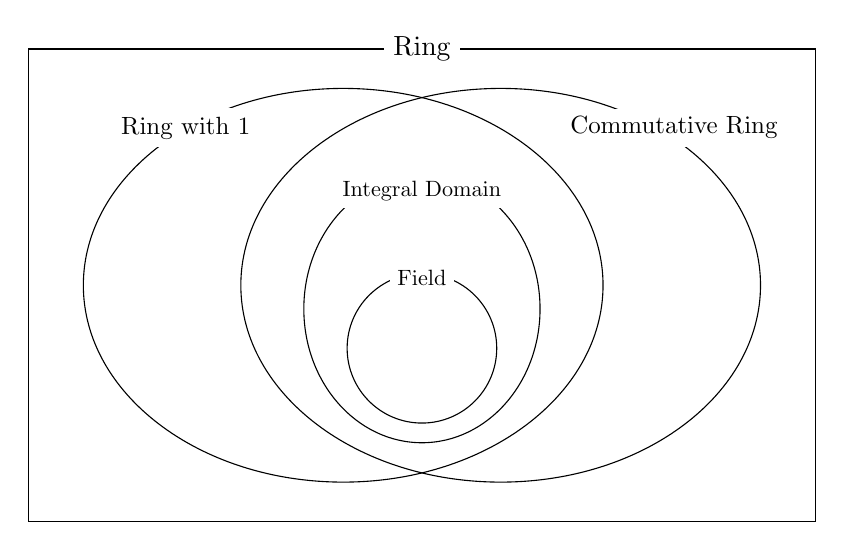
\begin{tikzpicture}
        \draw (0, 0) rectangle (10, 6);
        \node[fill=white] at (5, 6) {Ring};
        \draw (4, 3) ellipse (3.3 and 2.5);
        \draw (6, 3) ellipse (3.3 and 2.5);
        \draw (5, 2.7) ellipse (1.5 and 1.7);
        \draw (5, 2.2) circle (0.95);
        \node[fill=white,scale=0.9] at (2, 5) {Ring with 1};
        \node[fill=white,scale=0.9] at (8.2, 5) {Commutative Ring};
        \node[fill=white,scale=0.8] at (5, 4.2) {Integral Domain};
        \node[fill=white,scale=0.8] at (5, 3.1) {Field};
    \end{tikzpicture}
\end{center}

\thm. Every finite integral domain is a field.

\pf Let \(D = \{a_0, \dots, a_n\}\) be an integral domain. For nonzero \(a \in D\), consider the set \(aD = \{aa_0, aa_1, \dots, aa_n\}\). We show that \(aD = D\). Since \(D\) is finite, it is enough to show that \(aa_i \neq aa_j\) for \(i \neq j\). This is clear since \(D\) is an integral domain. Since \(1 \in aD\), \(\exists a_i \in D\) such that \(a a_i = 1\). So \(\exists a\inv = a_i\), concluding that \(D\) is a field. \qed

\pagebreak

\pf (Another) Let \(x \in D \bs \{0\}\). Then consider \(x, x^2, \dots\). Due to finiteness, \(x^n = x^m\) for two distinct \(n, m \in \N\). Then \(x^{n-m} = 1\) by cancellation. We conclude that \(x\) has an inverse. \qed

\cor. If \(p\) is prime, \(\Z_p\) is a field.

\subsection*{Characteristic of Ring}

\defn. \note{Characteristic}
\begin{enumerate}
    \item Let \(R\) be a ring. If there exists \(n \in \N\) such that \(na = 0\) for all \(a \in R\), then the least such integer \(n\) is called the \textbf{characteristic} of \(R\) and write \(\ch R = n\).
    \item If there does not exist such integer, we say that the characteristic of \(R\) is zero.
\end{enumerate}

\thm. Let \(R\) be a ring with unity, and let \(n \in \N\). Then \(\ch R = n\) if and only if \(n\) is the smallest positive integer such that \(n \cdot 1 = 0\).

\pf \note{\mimp} Trivial.

\note{\mimpd} For all \(a \in R\),
\[
    na = \overbrace{a + a + \cdots + a}^{n \text{ times}} = a(1 + 1 + \cdots + 1) = a(n \cdot 1) = a0 = 0.
\]
So \(\ch R = n\), since \(n\) is the smallest positive integer. \qed

\smallskip
